
\chapter{Design And Implementation}

The first step in this project was to choose a framework and type of website we wanted to build. We had two options : 
\begin{itemize}
	\item Static Website
	\item Dynamic Website
\end{itemize}
Dynamic Website provided us with great flexibility in the choice of programming language. It was much easier to build using existing libraries and tools. However, It was costly to deploy because an active server running the scripts on the back end as per the requests is needed. The programs to implement the various algorithms of numerical methods are not too complex and require no database.

On the other hand, static sites can be run on the client side but the lack of libraries specific to mathematical visualization and functions meant that we had to code a lot of it by ourselves. They are however free to deploy and serve.

We went with the static option and decided to use Jekyll, which is a static website generator. It utilizes markdown along with HTML and CSS to easily generate websites that are blog-like. The following figure show this.

\begin{figure}[h!]
	\centering
	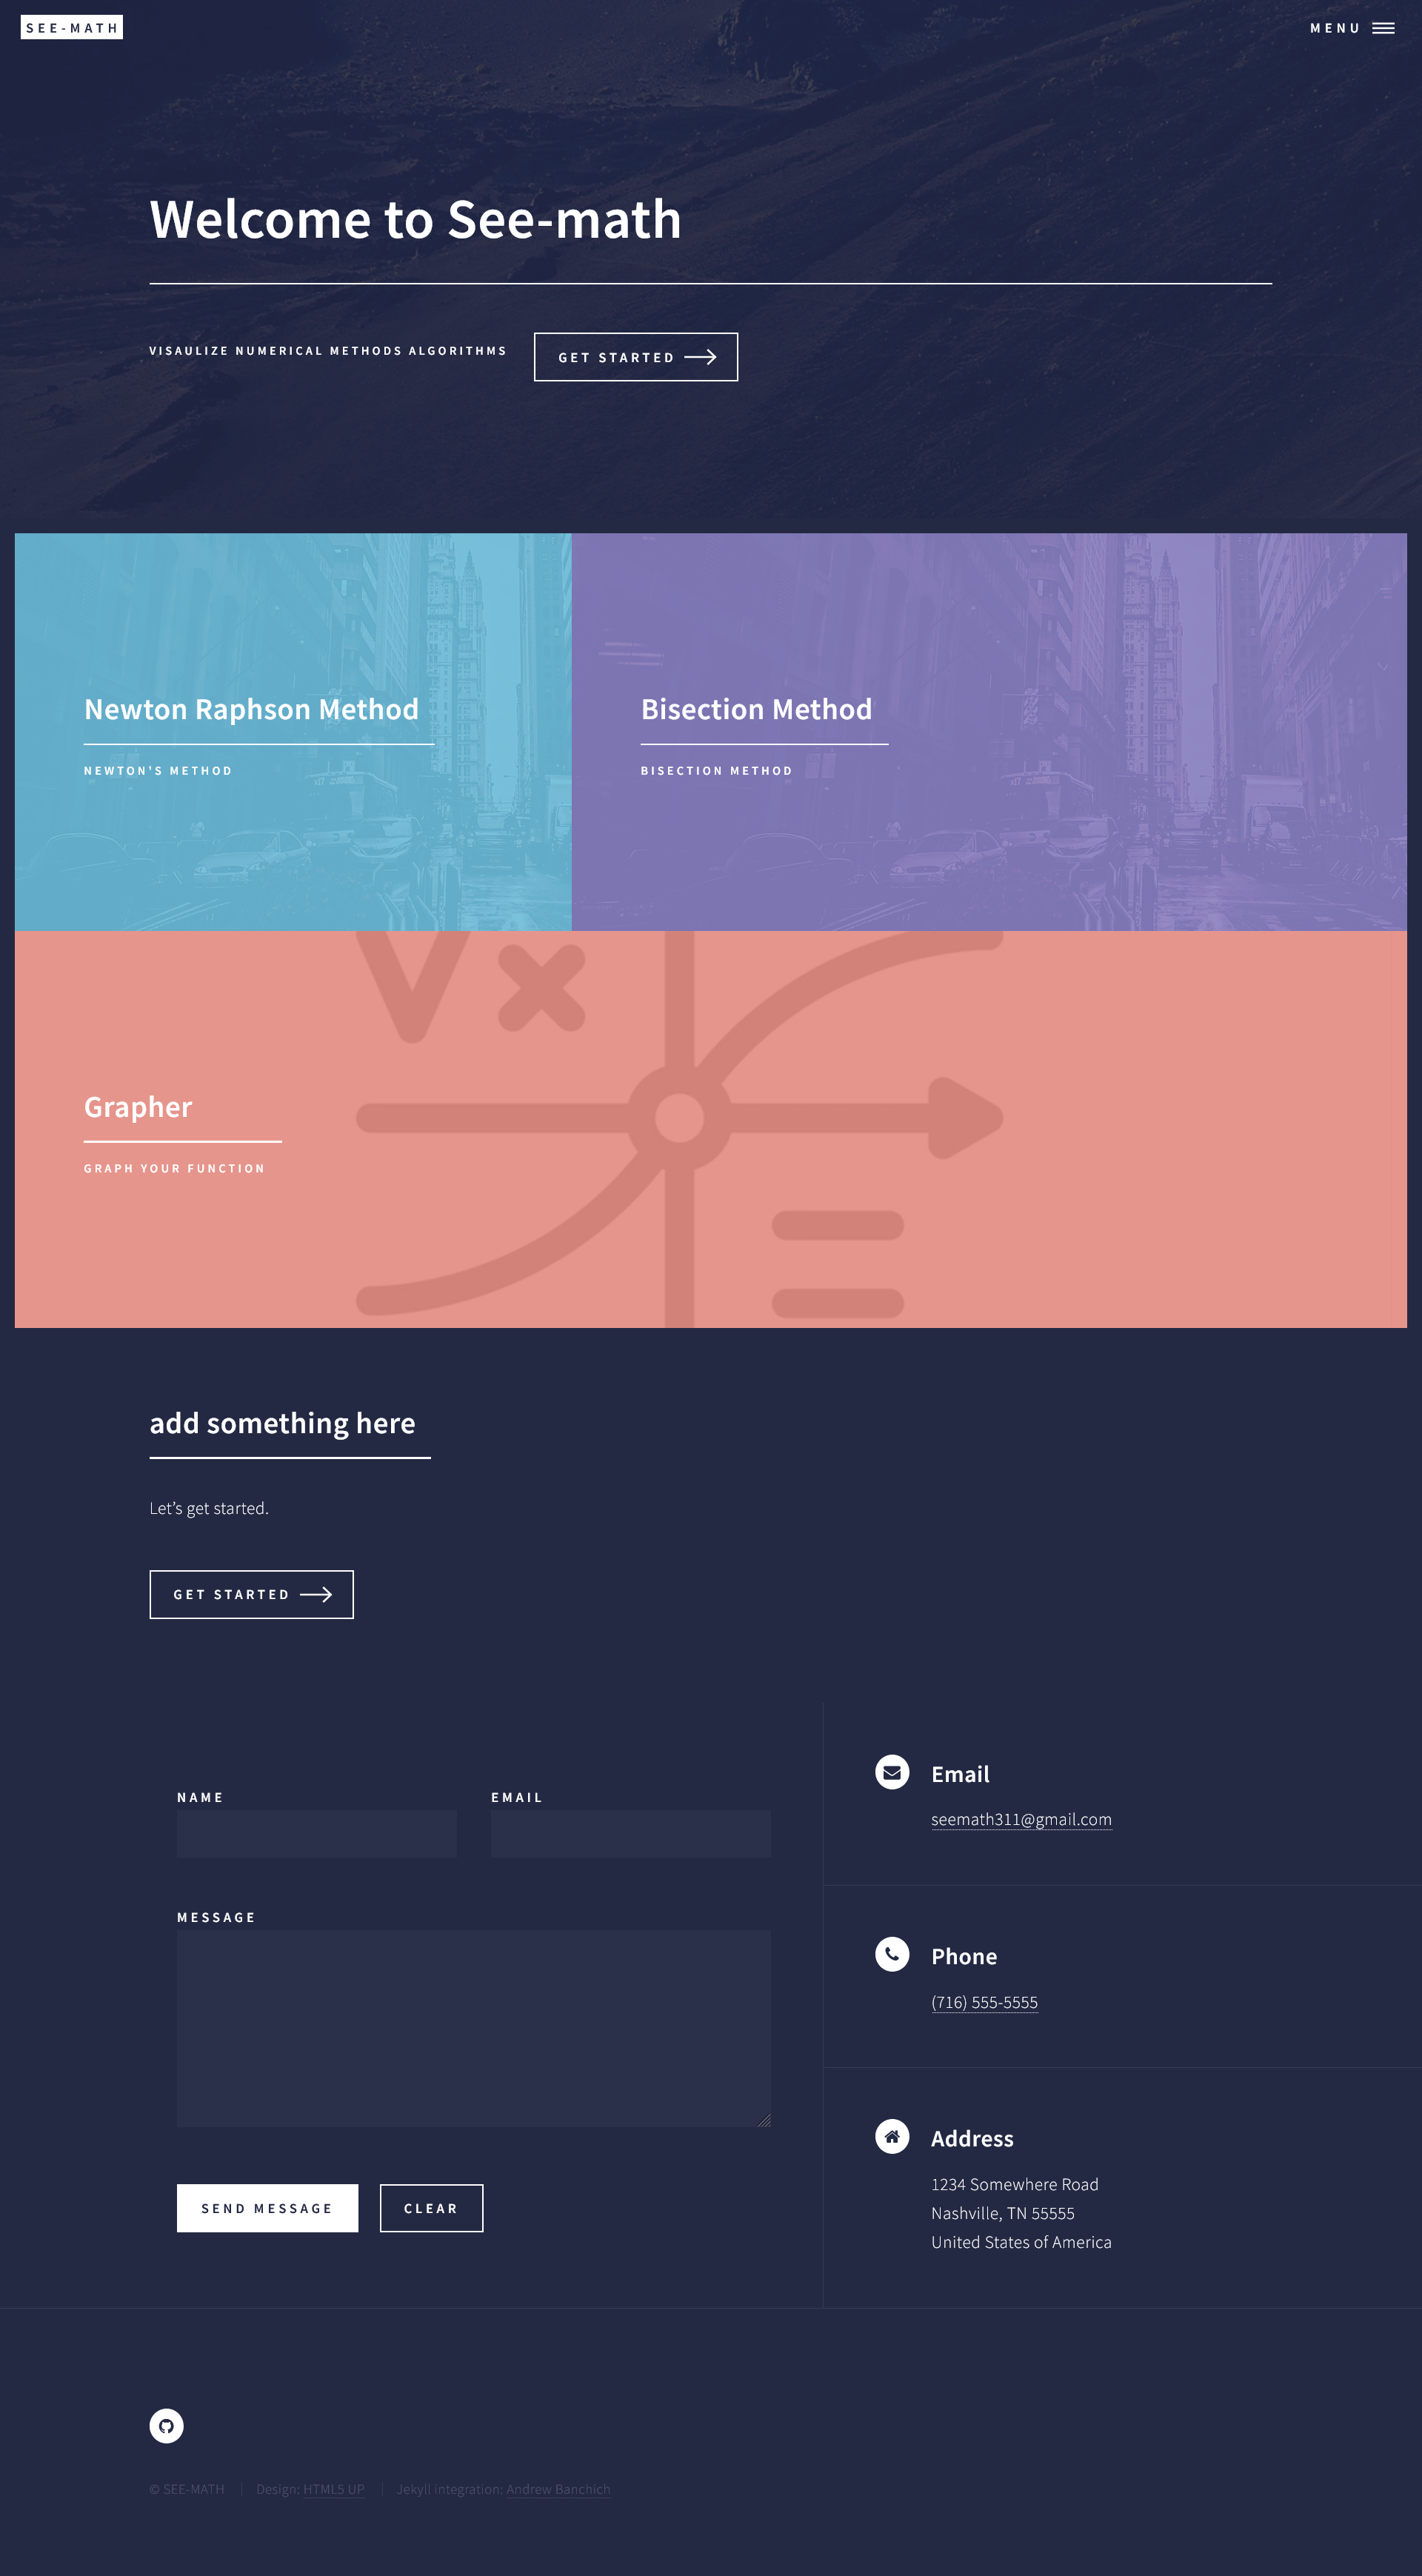
\includegraphics[width=0.8\linewidth]{seemath1}
	\caption{UI layout of website}
\end{figure}

\pagebreak
The next step was to design the method for getting user inputs, which are mathematical formulas in our case, and converting them to functions. We also needed to get a way to plot them and display the output. We utilized various libraries like 'math.js', 'mathjax.js', and 'plotly.js' to get the desired result.

\begin{figure}[h!]
	\centering
	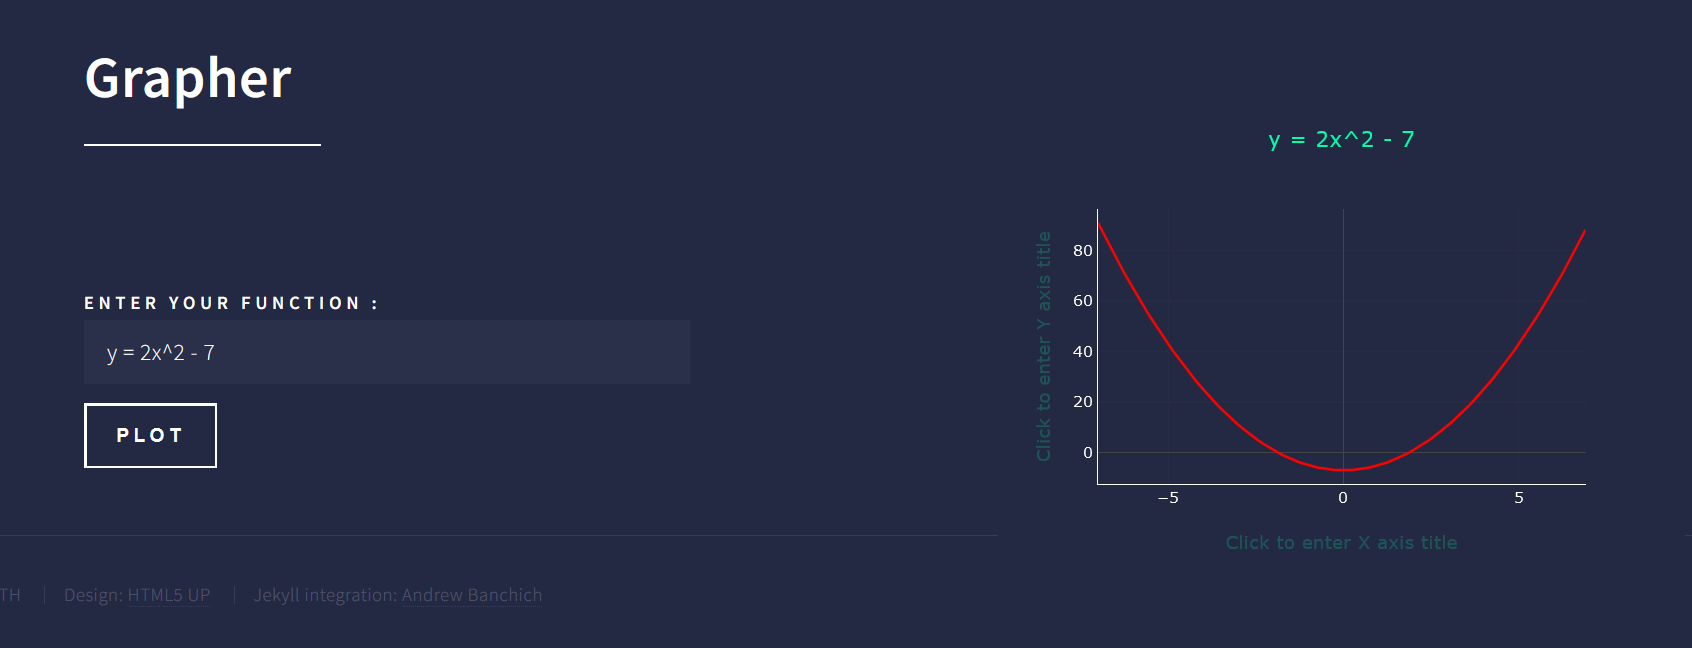
\includegraphics[width=0.89\linewidth]{seemath3}
	\caption{Input and Graphing Features}
\end{figure}

However, for getting step-wise solutions and visualizations associated with each iteration of algorithms like Bisection or Newton-Rhapson, we need a canvas-like library to be able to draw and remove geometrical objects. After extensive research, we found that 'JSXgraph' fitted the bill. we then began with implementing the algorithms and then the steps to visualize them in JS.

\begin{figure}[h!]
	\centering
	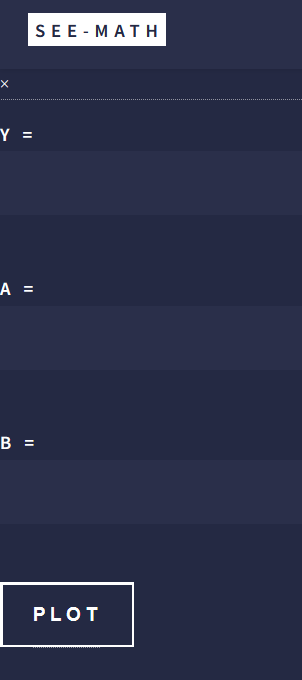
\includegraphics[width=0.24\linewidth]{seemath4}
	\caption{User Input for Bisection}
\end{figure}

\pagebreak
The graphs for both the methods are generated by using plot button. the next and animate button show the iterations with animation. Each graph can be panned, zoomed and interacted with. 
There are no zoom and pan feature in the JSXgraph library. Thus, we had to look at other methods. We utilized the fact that we could change the boundary box of the graph and changed it in a slow and controlled way to slowly transition from one state to another.
\begin{figure}[h!]
	\centering
	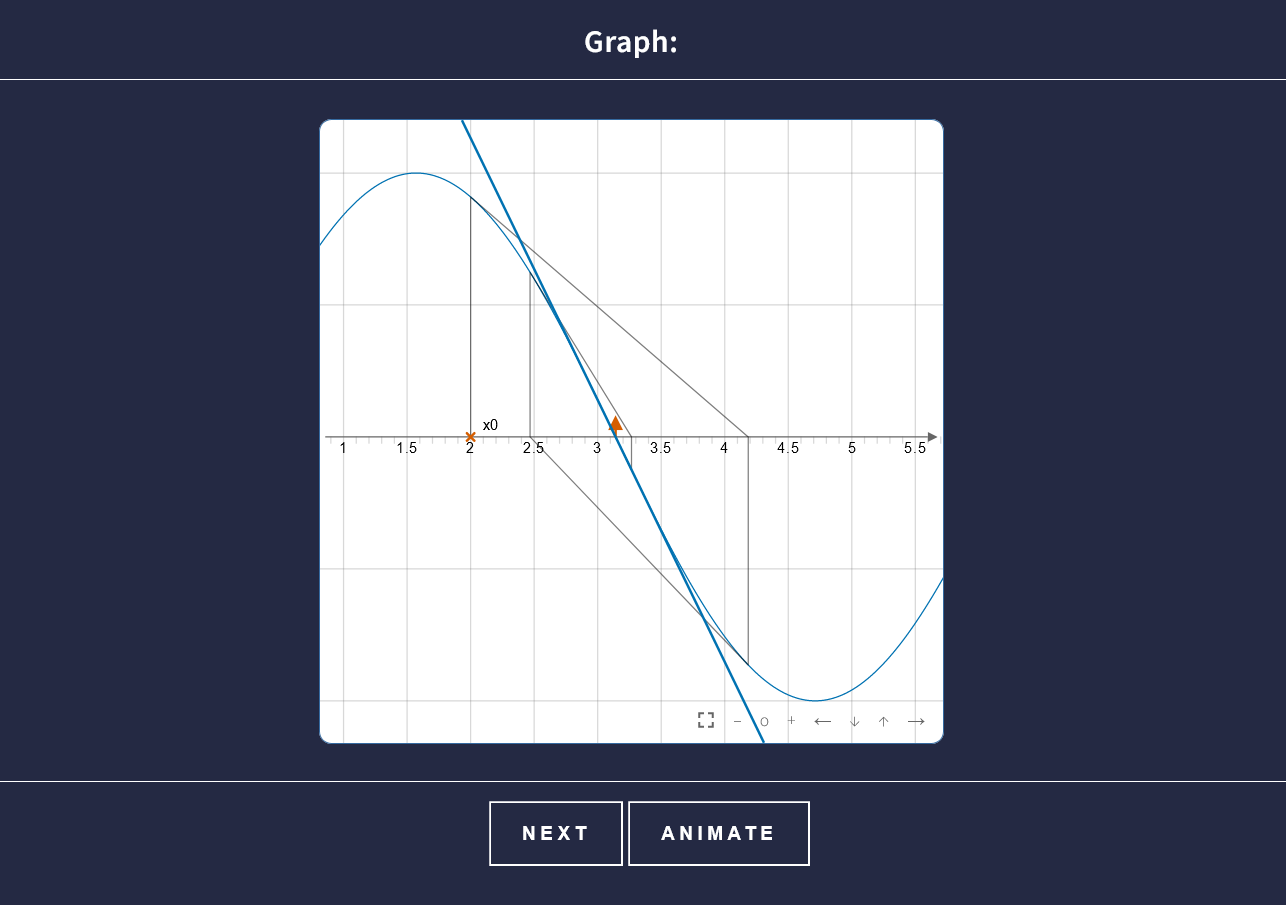
\includegraphics[width=0.89\linewidth]{seemath6}
	\caption{Newton Rhapson Method}
\end{figure}

\begin{figure}[h!]
\centering
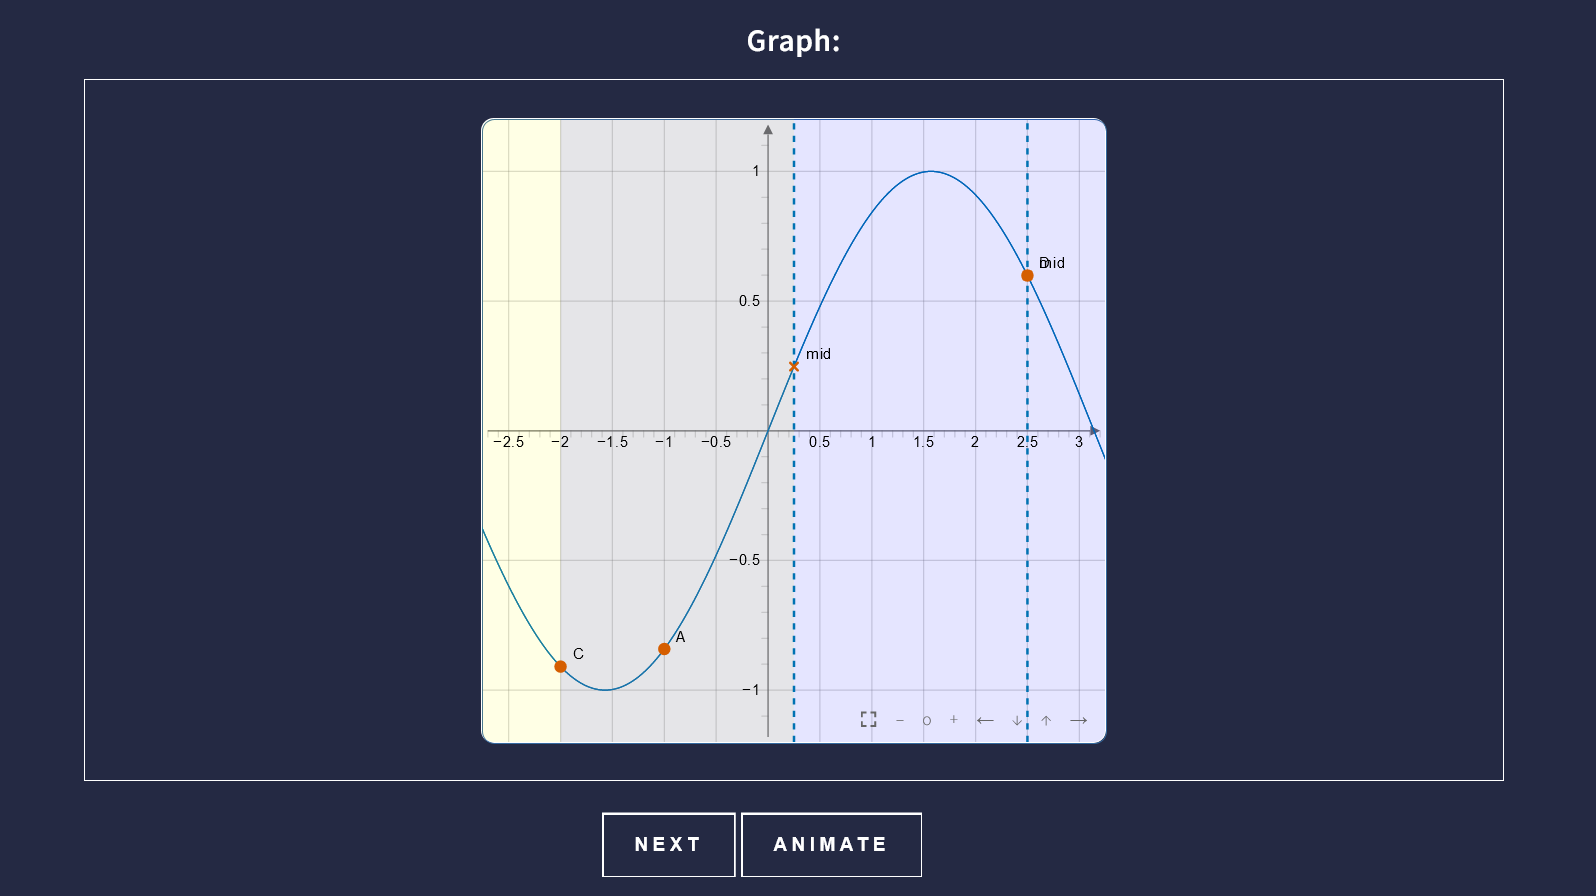
\includegraphics[width=0.89\linewidth]{seemath7}
\caption{Bisection Method}
\end{figure}

\pagebreak
To make getting feedback and suggestions easier, we added a contact form. Since there is no dynamic elements in our website or a central server to receive the feedback and process it. We utilized a service known as 'Formspree'\cite{form} to get emails containing the feedback.

\begin{figure}[h!]
	\centering
	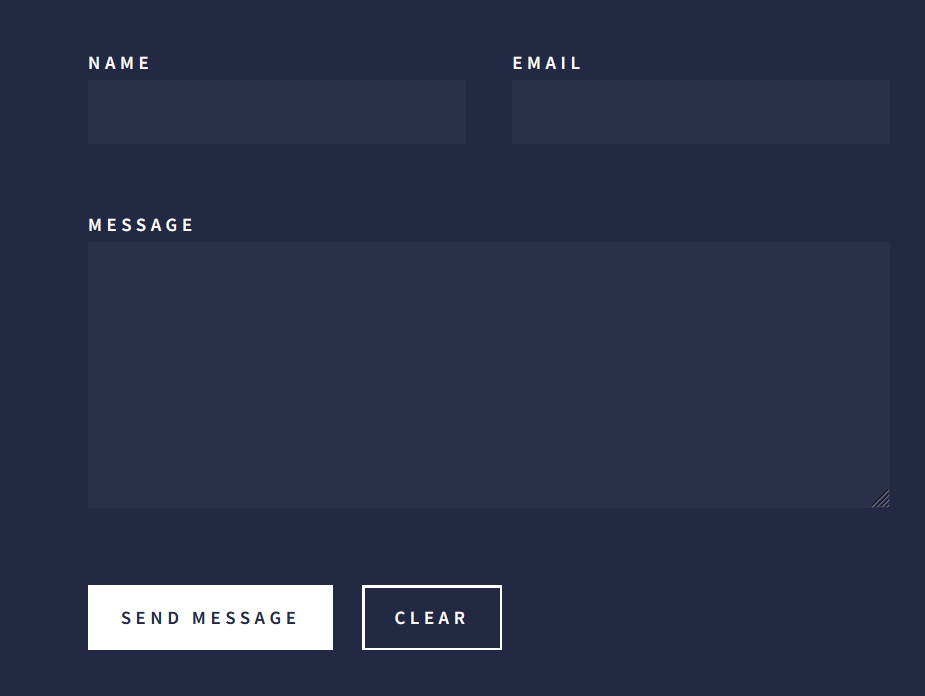
\includegraphics[width=0.5\linewidth]{seemath5}
	\caption{Feedback Form}
\end{figure}

